% **************************************************************************************************
% **************************************************************************************************
\newsection{Datasets}{method:datasets}
For timbre estimation of target instruments from a mixture, a task related to source separation, so-called \textit{multi-track datasets} are required for training of the \glspl{dnn}. Such datasets provide the audio recordings of the individual tracks, also referred to as \textit{sources}, which make up a song when added together. Usually, these tracks are not processed in any way and are stored as mono files. As a positive side effect, access to the individual sources allows extensive data augmentation, because the sources can be processed independently and random mixes can be created from these single-instrument tracks (more about that in Section~\ref{sec:method:preprocessing}). In the course of this work, a combination of three multi-track datasets was used. Furthermore, a large music tagging dataset was utilized for pre-training of all models. This music tagging dataset already comes with a predefined split. However, the multi-track datasets were randomly divided into training, validation and test sets containing \SI{65}{\percent}, \SI{17.5}{\percent} and \SI{17.5}{\percent} of all songs, respectively. We made the decision to split the multi-track datasets at random for the sake of simplicity. Be aware that this practice can potentially lead to overoptimistic results if songs from the same artist or album are contained in multiple splits.

\newsubsection{MTG-Jamendo}{method:datasets:jamendo}
The music tagging dataset \textit{MTG-Jamendo}~\cite{bogdanov2019jamendo} was used for pre-training. It features 55,701 free\footnote{Since music is usually copyright protected and therefore hard to collect, large-scale datasets for \gls{mir} are rare. To get around copyright, many creators of music datasets use royalty-free tracks or publish pre-computed features instead of audio files.} full-length music tracks from the \textit{Jamendo}\footnote{https://www.jamendo.com/} platform. Tags are provided by the content uploaders and cover genre, instruments and mood/theme. Only the 50 most popular tags were used for pre-training of the convolutional layers of all models. Although these tags include only a few instrument labels but plenty of genre and mood/theme labels, we hope that, after pre-training, the learned music tagging skills can easily be transferred to \gls{ir}.\\

It is worth mentioning that, besides MTG-Jamendo, there are various other large music datasets, which could be used for pre-training. The \textit{Million Song Dataset}~\cite{bertin2011msd} is by far the biggest music dataset available, containing audio features and metadata for one million tracks. The audio files are not included in the dataset, but there is the possibility to download 30-second previews from \textit{7digital}\footnote{https://www.7digital.com/}. Unfortunately, it is impossible to get an API key for the website at the moment. \textit{MagnaTagATune}~\cite{law2009mtat} is a collection of 25,863 music clips. The clips are 29 seconds long and have been extracted from 5223 songs. A major downside is the low audio quality of the tracks -- MP3 files with only \SI{16}{\kilo\hertz} sample rate and \SI{32}{kbps} bit rate. Finally, there is \textit{AudioSet}~\cite{gemmeke2017audioset}, a huge dataset of 2.1 million annotated YouTube videos for audio event detection. Classes cover a wide range of environmental sounds, however, music-related tags like instrumentation and genre are represented as well. To avoid copyright issues, the creators of the dataset only provide links to the videos instead of audio files. To demonstrate the potential of AudioSet, the authors of~\cite{kong2020panns} pre-trained different \glspl{dnn} on AudioSet and reported state-of-the-art results on a couple of audio classification tasks after fine-tuning on smaller datasets. In order not to spend too much time on pre-training, the decision was made to stick with MTG-Jamendo instead of conducting further experiments with the datasets mentioned above.

\newsubsection{MedleyDB}{method:datasets:medleydb}
\textit{MedleyDB}~\cite{bittner2014medleydb} is a multi-track dataset of licence-free music. While the creators of the dataset primarily focused on melody extraction, instrument annotations are also provided, making the dataset suitable for \gls{ir}. MedleyDB contains the individual instrument tracks of 122 songs from various genres. All files are stored in the uncompressed WAV format with \SI{44.1}{\kilo\hertz} sample rate and a bit depth of 16. In 2016, \textit{MedleyDB 2.0}~\cite{bittner2016medleydb2} was released, adding 74 new songs. In this work, we merged MedleyDB and MedleyDB 2.0. Hereafter, for the sake of simplicity, the combination of both datasets will be referred to as MedleyDB. Since not all songs have been recorded in a clean studio environment, some tracks exhibit a considerable amount of crosstalk. After listening to every track, tracks with severe crosstalk have been discarded, as training with bleeding sources would introduce errors. After this cleaning procedure, 134 songs remain. In Fig.~\ref{fig:stats-medleydb}, the distribution of instrument families and instruments -- after mapping the original labels of MedleyDB according to the hierarchical taxonomy introduced in Section~\ref{sec:method:taxonomy} -- are depicted.\\
\begin{figure}
	\centering%
	\subfigure[Number of sources per family]{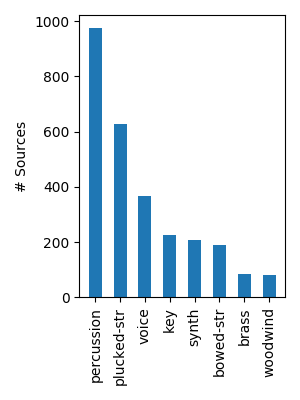
\includegraphics[width=0.35\textwidth]{\pwd/figs/families_medleydb_all.png}}%
	\subfigure[Number of sources per instrument]{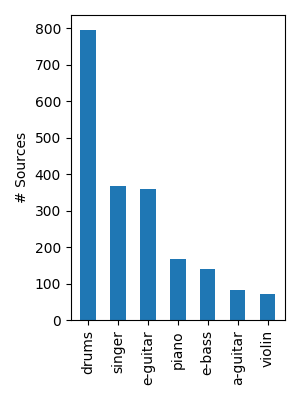
\includegraphics[width=0.35\textwidth]{\pwd/figs/classes_medleydb_all.png}}%
	\caption{Distribution of instrument families and instruments in MedleyDB.}\label{fig:stats-medleydb}
\end{figure}

\newsubsection{Mixing Secrets}{method:datasets:mixingsecrets}
The \textit{Mixing Secrets}~\cite{gururani2017mixingsecrets} dataset is inspired by MedleyDB and therefore has a similar structure. Like its role model, Mixing Secrets contains exclusively free music. All tracks have been aggregated from the \textit{Mixing Secrets For The Small Studio}\footnote{https://www.cambridge-mt.com/ms/mtk/} website, which provides hundreds of free multi-track projects for non-commercial use. In order to download the audio, the creators of the dataset published URLs to all files. Since several links did not work and some have been removed due to massive crosstalk, the final dataset counts 125 songs. The distribution of sources is depicted in Fig.~\ref{fig:stats-mixingsecrets}.\\
\begin{figure}
	\centering%
	\subfigure[Number of sources per family]{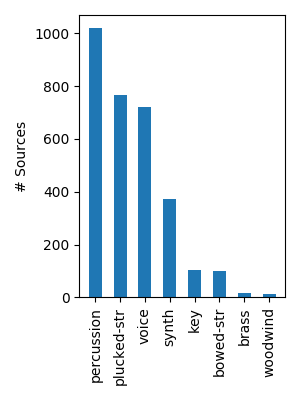
\includegraphics[width=0.35\textwidth]{\pwd/figs/families_mixing-secrets_all.png}}%
	\subfigure[Number of sources per instrument]{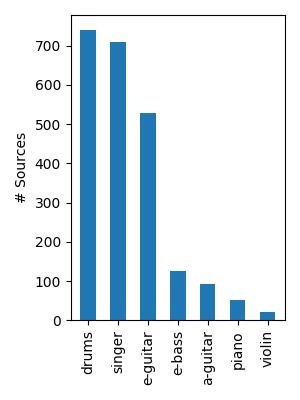
\includegraphics[width=0.35\textwidth]{\pwd/figs/classes_mixing-secrets_all.png}}%
	\caption{Distribution of instrument families and instruments in Mixing Secrets.}\label{fig:stats-mixingsecrets}
\end{figure}

\newsubsection{Slakh}{method:datasets:slakh}
\textit{Slakh}~\cite{manilow2019slakh}, containing 2,100 songs, is by far the largest multi-track dataset available. All tracks have been synthesized from the \textit{Lakh MIDI Dataset v0.1}\footnote{https://colinraffel.com/projects/lmd/} using virtual instruments. For this reason, most instruments sound quite \enquote{cheap} and unnatural. Since training data should be as close as possible to real-world data when training \gls{ml} algorithms, the Slakh dataset is rather suboptimal. However, we decided to use Slakh anyhow because we hoped that its huge size can compensate for this disadvantage. Fig.~\ref{fig:stats-slakh} illustrates the distribution of instrument families and instruments of this dataset.\\
\begin{figure}
	\centering%
	\subfigure[Number of sources per family]{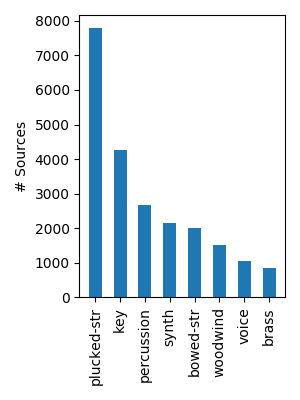
\includegraphics[width=0.35\textwidth]{\pwd/figs/families_slakh_all.png}}%
	\subfigure[Number of sources per instrument]{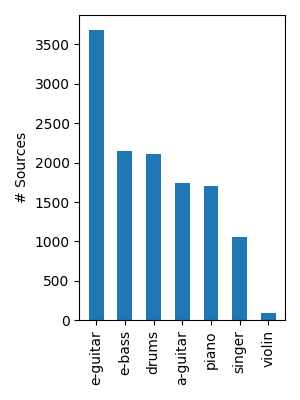
\includegraphics[width=0.35\textwidth]{\pwd/figs/classes_slakh_all.png}}%
	\caption{Distribution of instrument families and instruments in Slakh.}\label{fig:stats-slakh}
\end{figure}

